\documentclass{article}
\usepackage{graphicx}
\usepackage[margin=1in]{geometry}

\begin{document}

\begin{table}
\centering
\caption{Median Reduced $\chi^2$: 0.95 -- Maximum-Likelihood Reduced $\chi^2$: 1.06}
\begin{tabular}{| c | c | c |}
\hline
Parameter & Median and $1 \sigma$ Values & Maximum-Likelihood \\
\hline
$P$ (days) & $71.69007^{+0.00036}_{-0.00032}$ & $71.69007$ \\
\hline
$t_{tran}$ (days) & $43072.579^{+0.036}_{-0.039}$ & $43072.585$ \\
\hline
$K_1$ (km/s) & $30.075^{+0.071}_{-0.070}$ & $30.104$ \\
\hline
$\gamma_{1} (km/s)$ & $1.88^{+0.33}_{-0.33}$ & $1.82$ \\
\hline
$\gamma_{2} (km/s)$ & $1.79^{+0.24}_{-0.24}$ & $1.72$ \\
\hline
$\gamma_{3} (km/s)$ & $1.27^{+0.52}_{-0.52}$ & $1.09$ \\
\hline
$\gamma_{4} (km/s)$ & $0.72^{+0.13}_{-0.13}$ & $0.73$ \\
\hline
$\gamma_{5} (km/s)$ & $0.981^{+0.076}_{-0.076}$ & $0.983$ \\
\hline
$\gamma_{6} (km/s)$ & $0.68^{+0.13}_{-0.13}$ & $0.73$ \\
\hline
$\gamma_{7} (km/s)$ & $0.39^{+0.11}_{-0.12}$ & $0.45$ \\
\hline
$\sigma^2_{j} (km/s)^2$ & $0.043^{+0.073}_{-0.032}$ & $0.035$ \\
\hline
$M_{error, 1} $ & $0.29^{+0.24}_{-0.12}$ & $0.17$ \\
\hline
$M_{error, 2} $ & $0.97^{+0.39}_{-0.25}$ & $0.89$ \\
\hline
$M_{error, 3} $ & $2.0^{+2.5}_{-1.0}$ & $1.2$ \\
\hline
$M_{error, 4} $ & $1.04^{+0.38}_{-0.27}$ & $1.02$ \\
\hline
$M_{error, 5} $ & $0.68^{+0.16}_{-0.13}$ & $0.71$ \\
\hline
$M_{error, 6} $ & $0.67^{+0.51}_{-0.27}$ & $0.46$ \\
\hline
$M_{error, 7} $ & $0.91^{+0.75}_{-0.41}$ & $0.86$ \\
\hline
\end{tabular}
\end{table}

\clearpage

\begin{figure}[!htb]
\centering
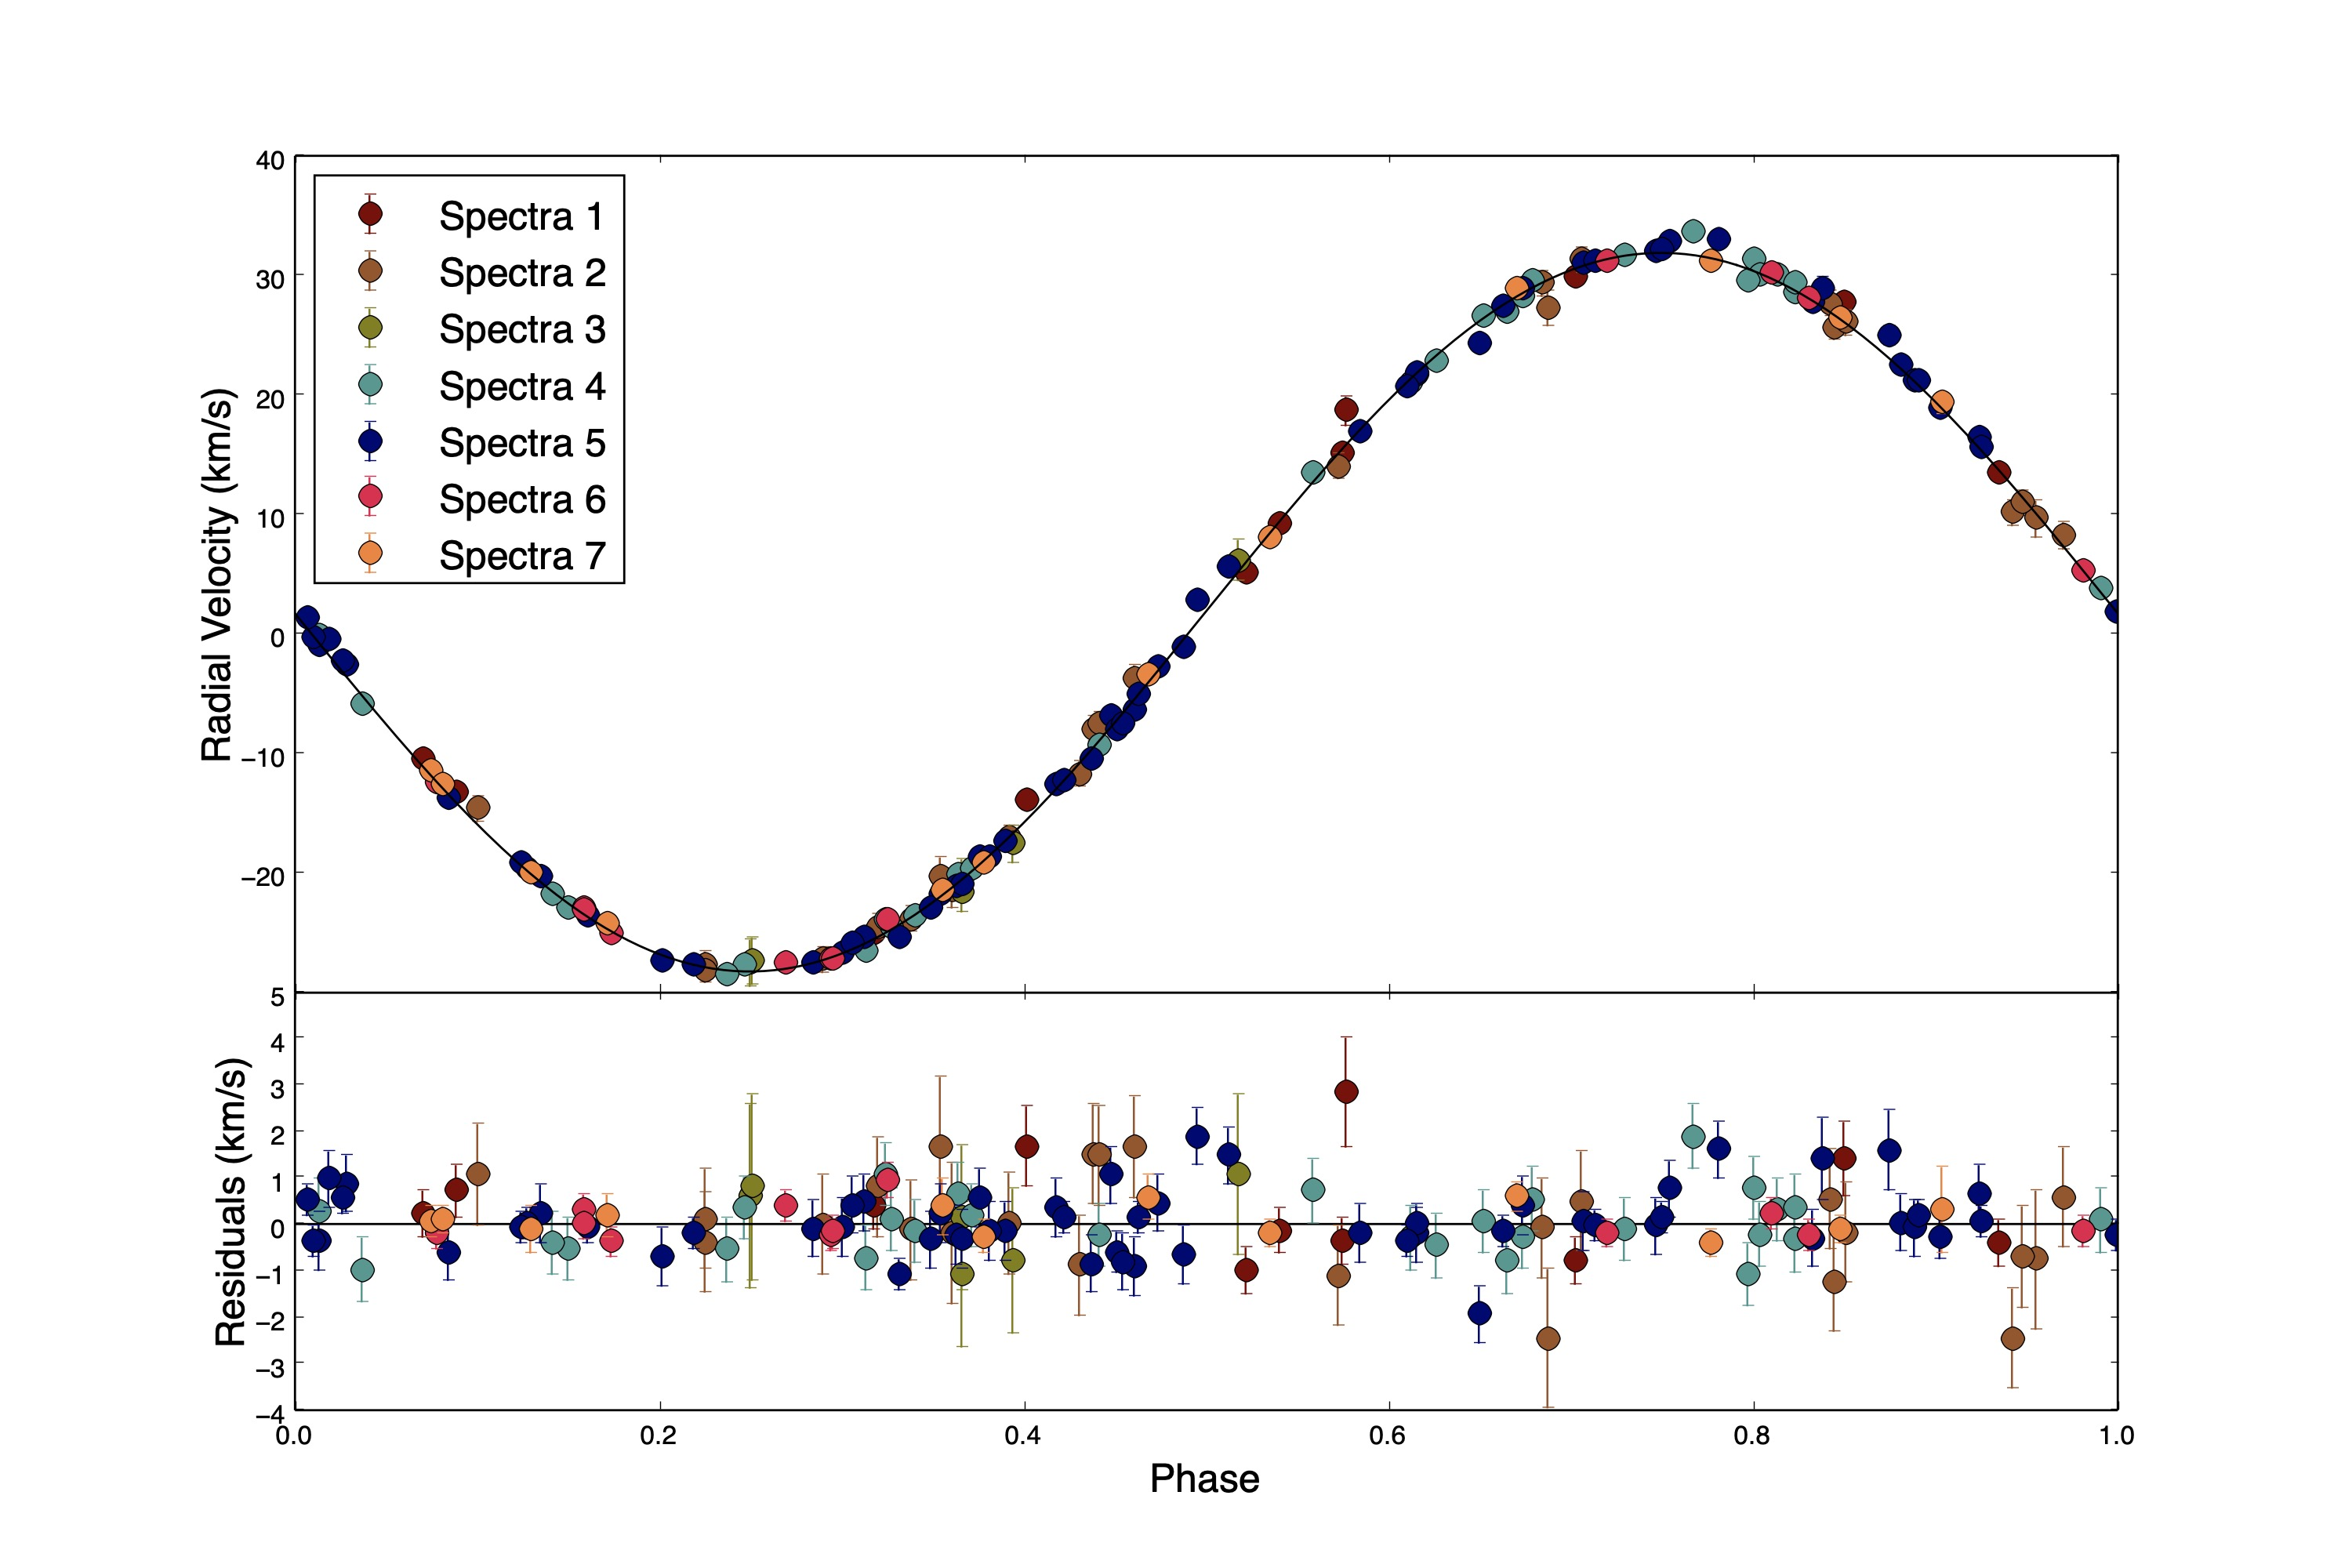
\includegraphics[width=0.9\textwidth]{RVfit_meds_100000_FixedEcc.jpg}
\caption{RV fit to median MCMC parameters. RMS residual velocity of 0.77 $\rm{km \: s^{-1}}$.}

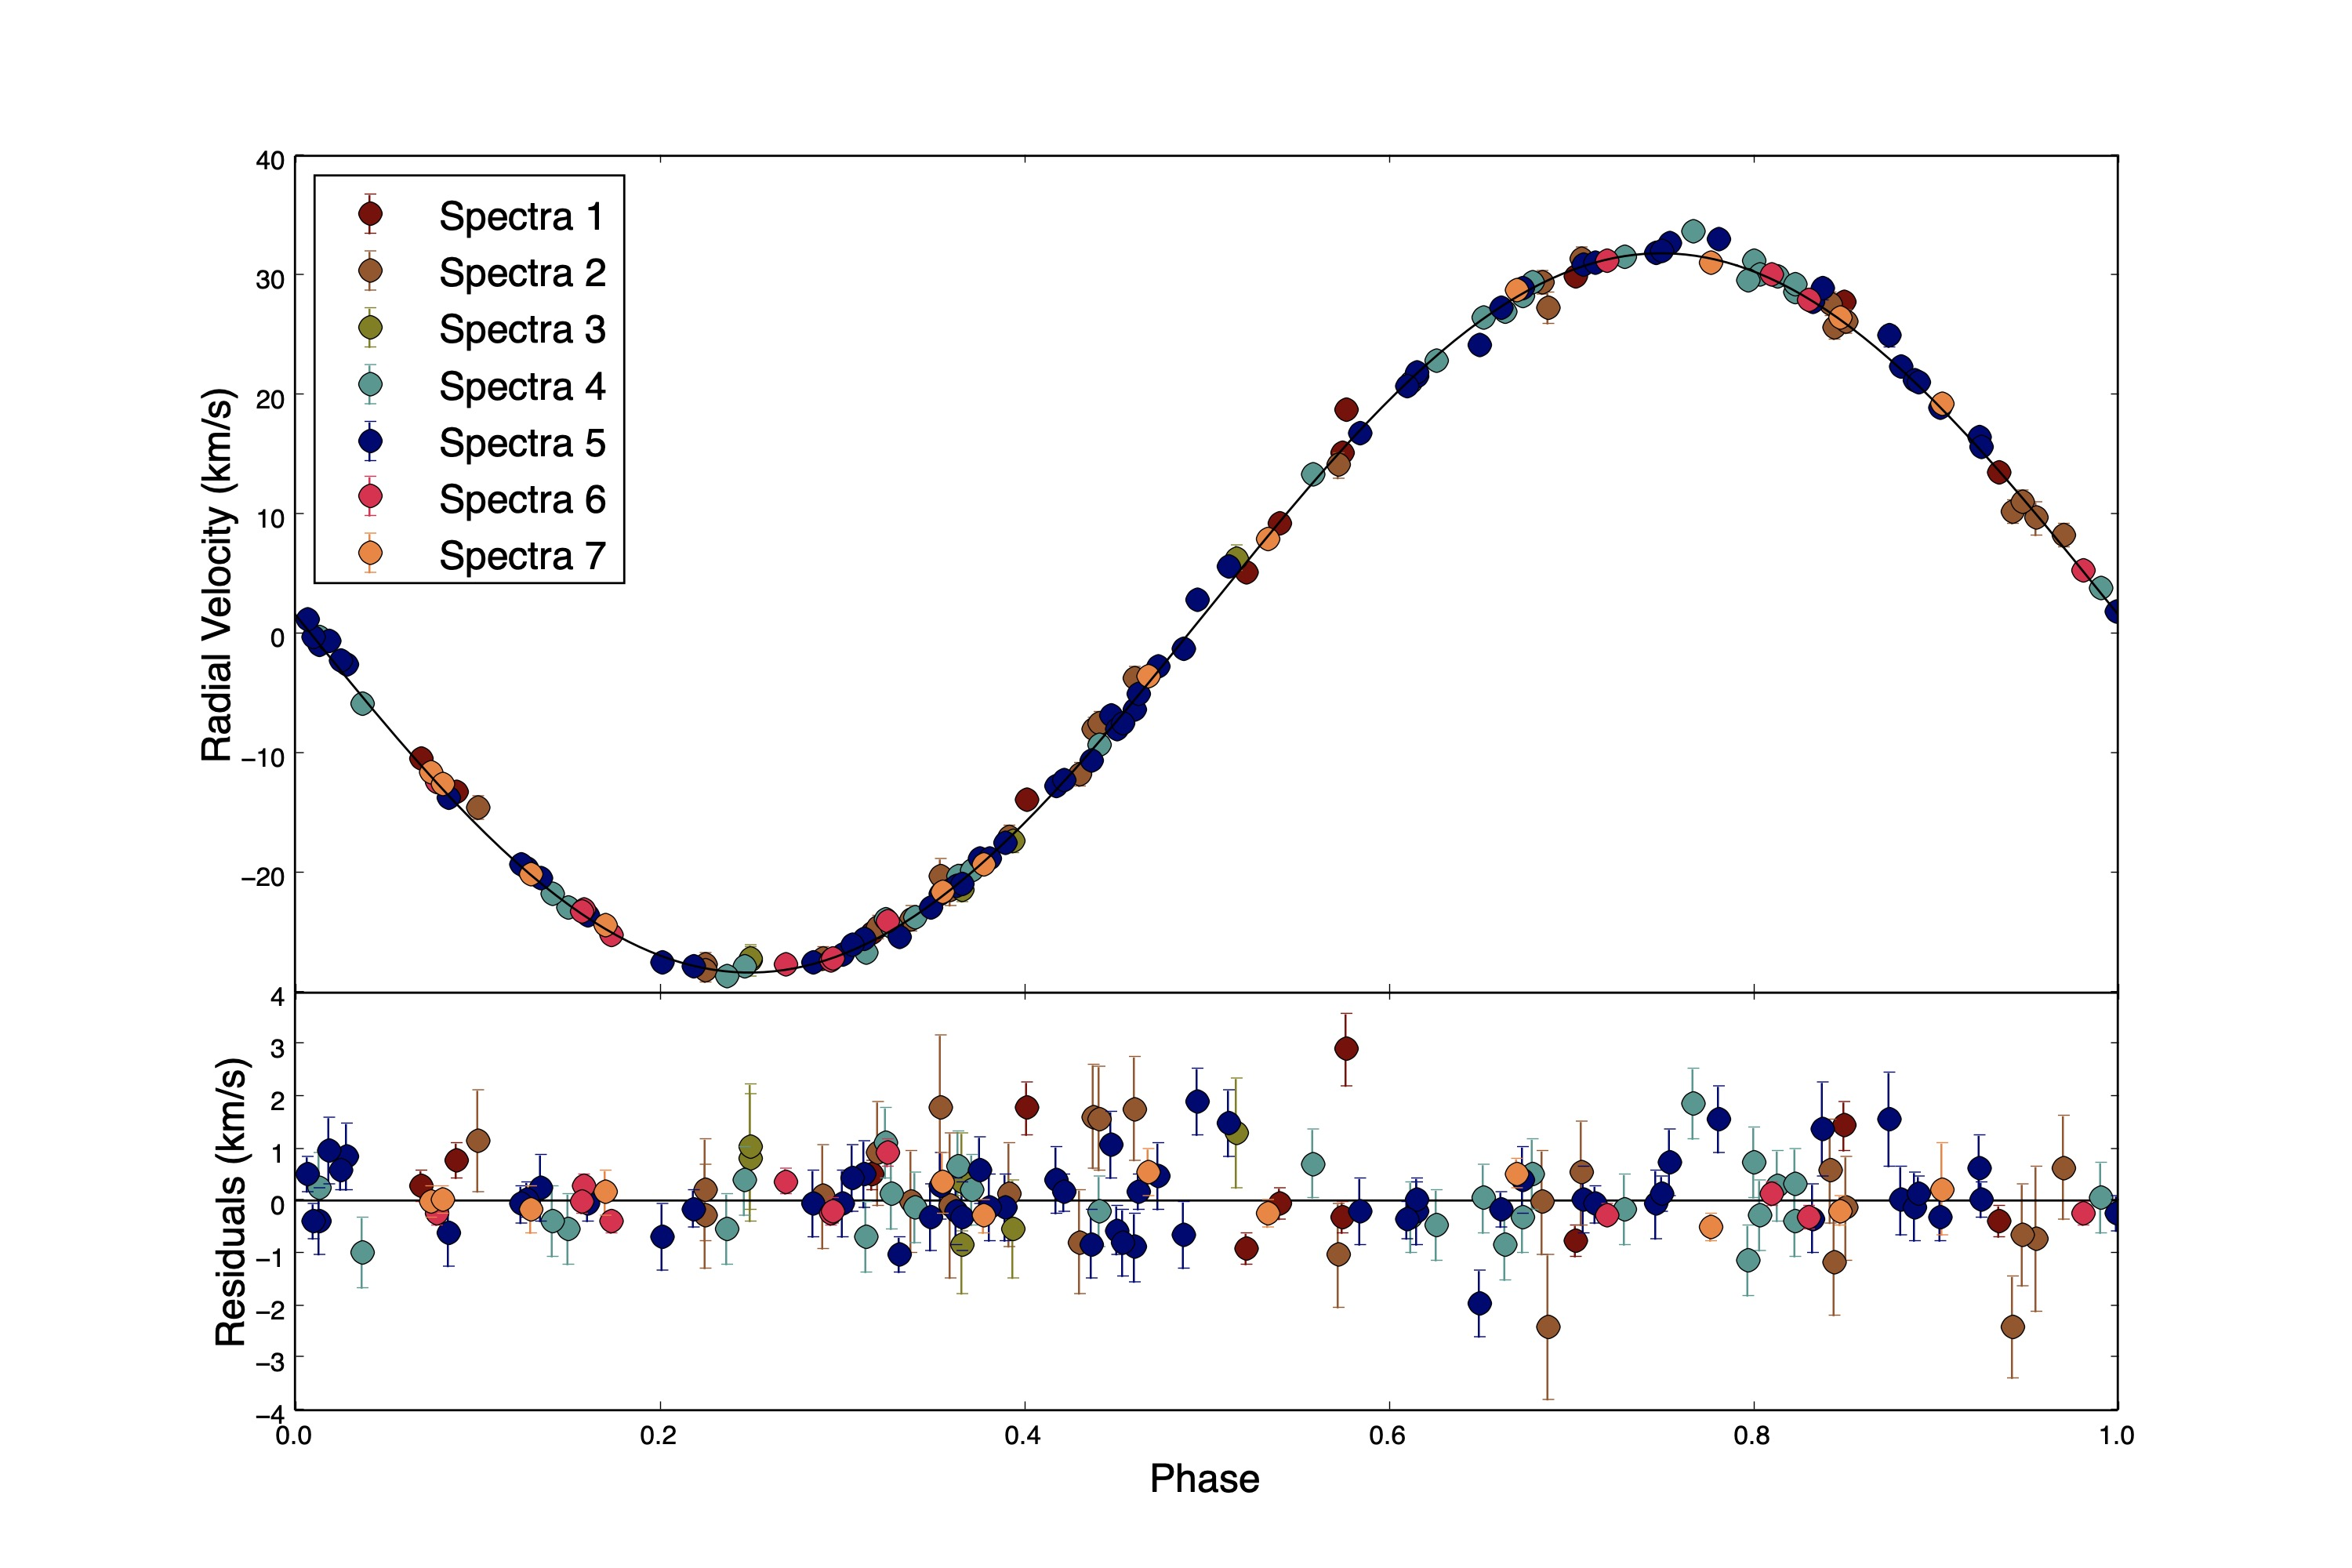
\includegraphics[width=0.9\textwidth]{RVfit_best_100000_FixedEcc.jpg}
\caption{RV fit to maximum-likelihood MCMC parameters. RMS residual velocity of 0.78 $\rm{km \: s^{-1}}$.}
\end{figure}


\begin{figure}[!htb]
\centering
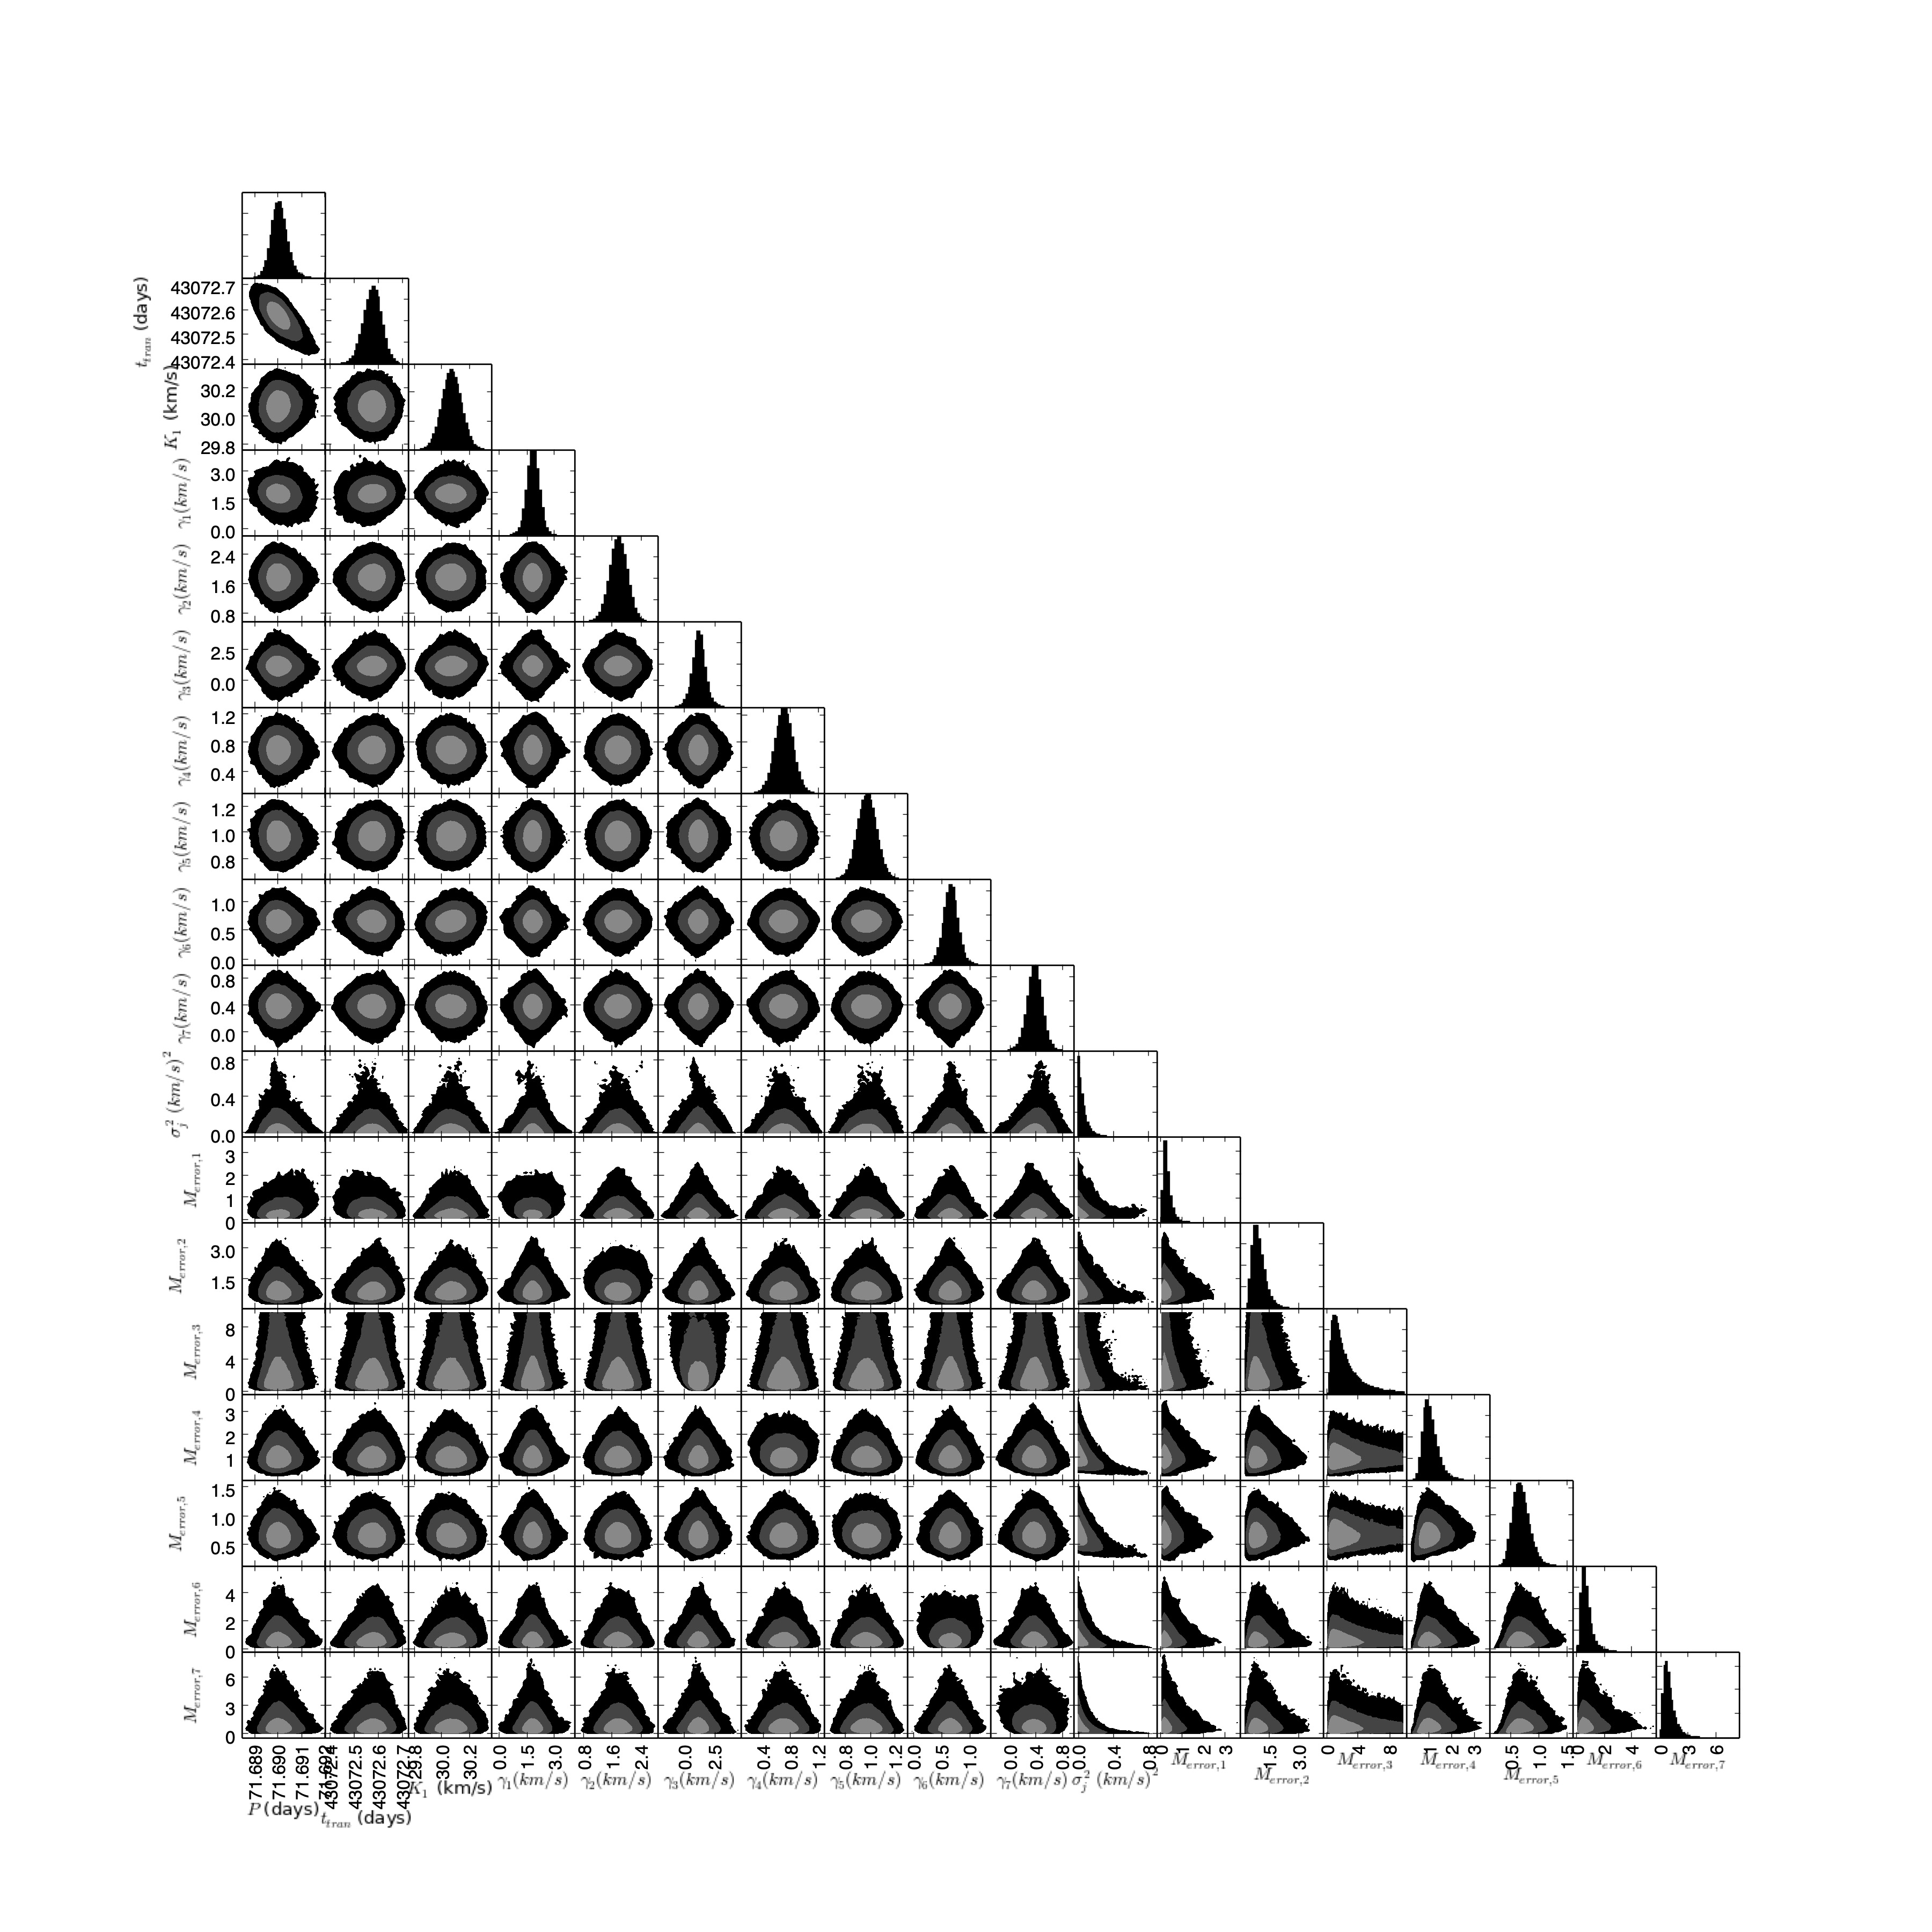
\includegraphics[width=\textwidth]{corner_100000_FixedEcc.jpg}
\caption{Contour plots showing the $1 \sigma$, $2 \sigma$, and $3 \sigma$ constraints on pairs of parameters for the MCMC model.}
\end{figure}


\begin{figure}[!htb]
\centering
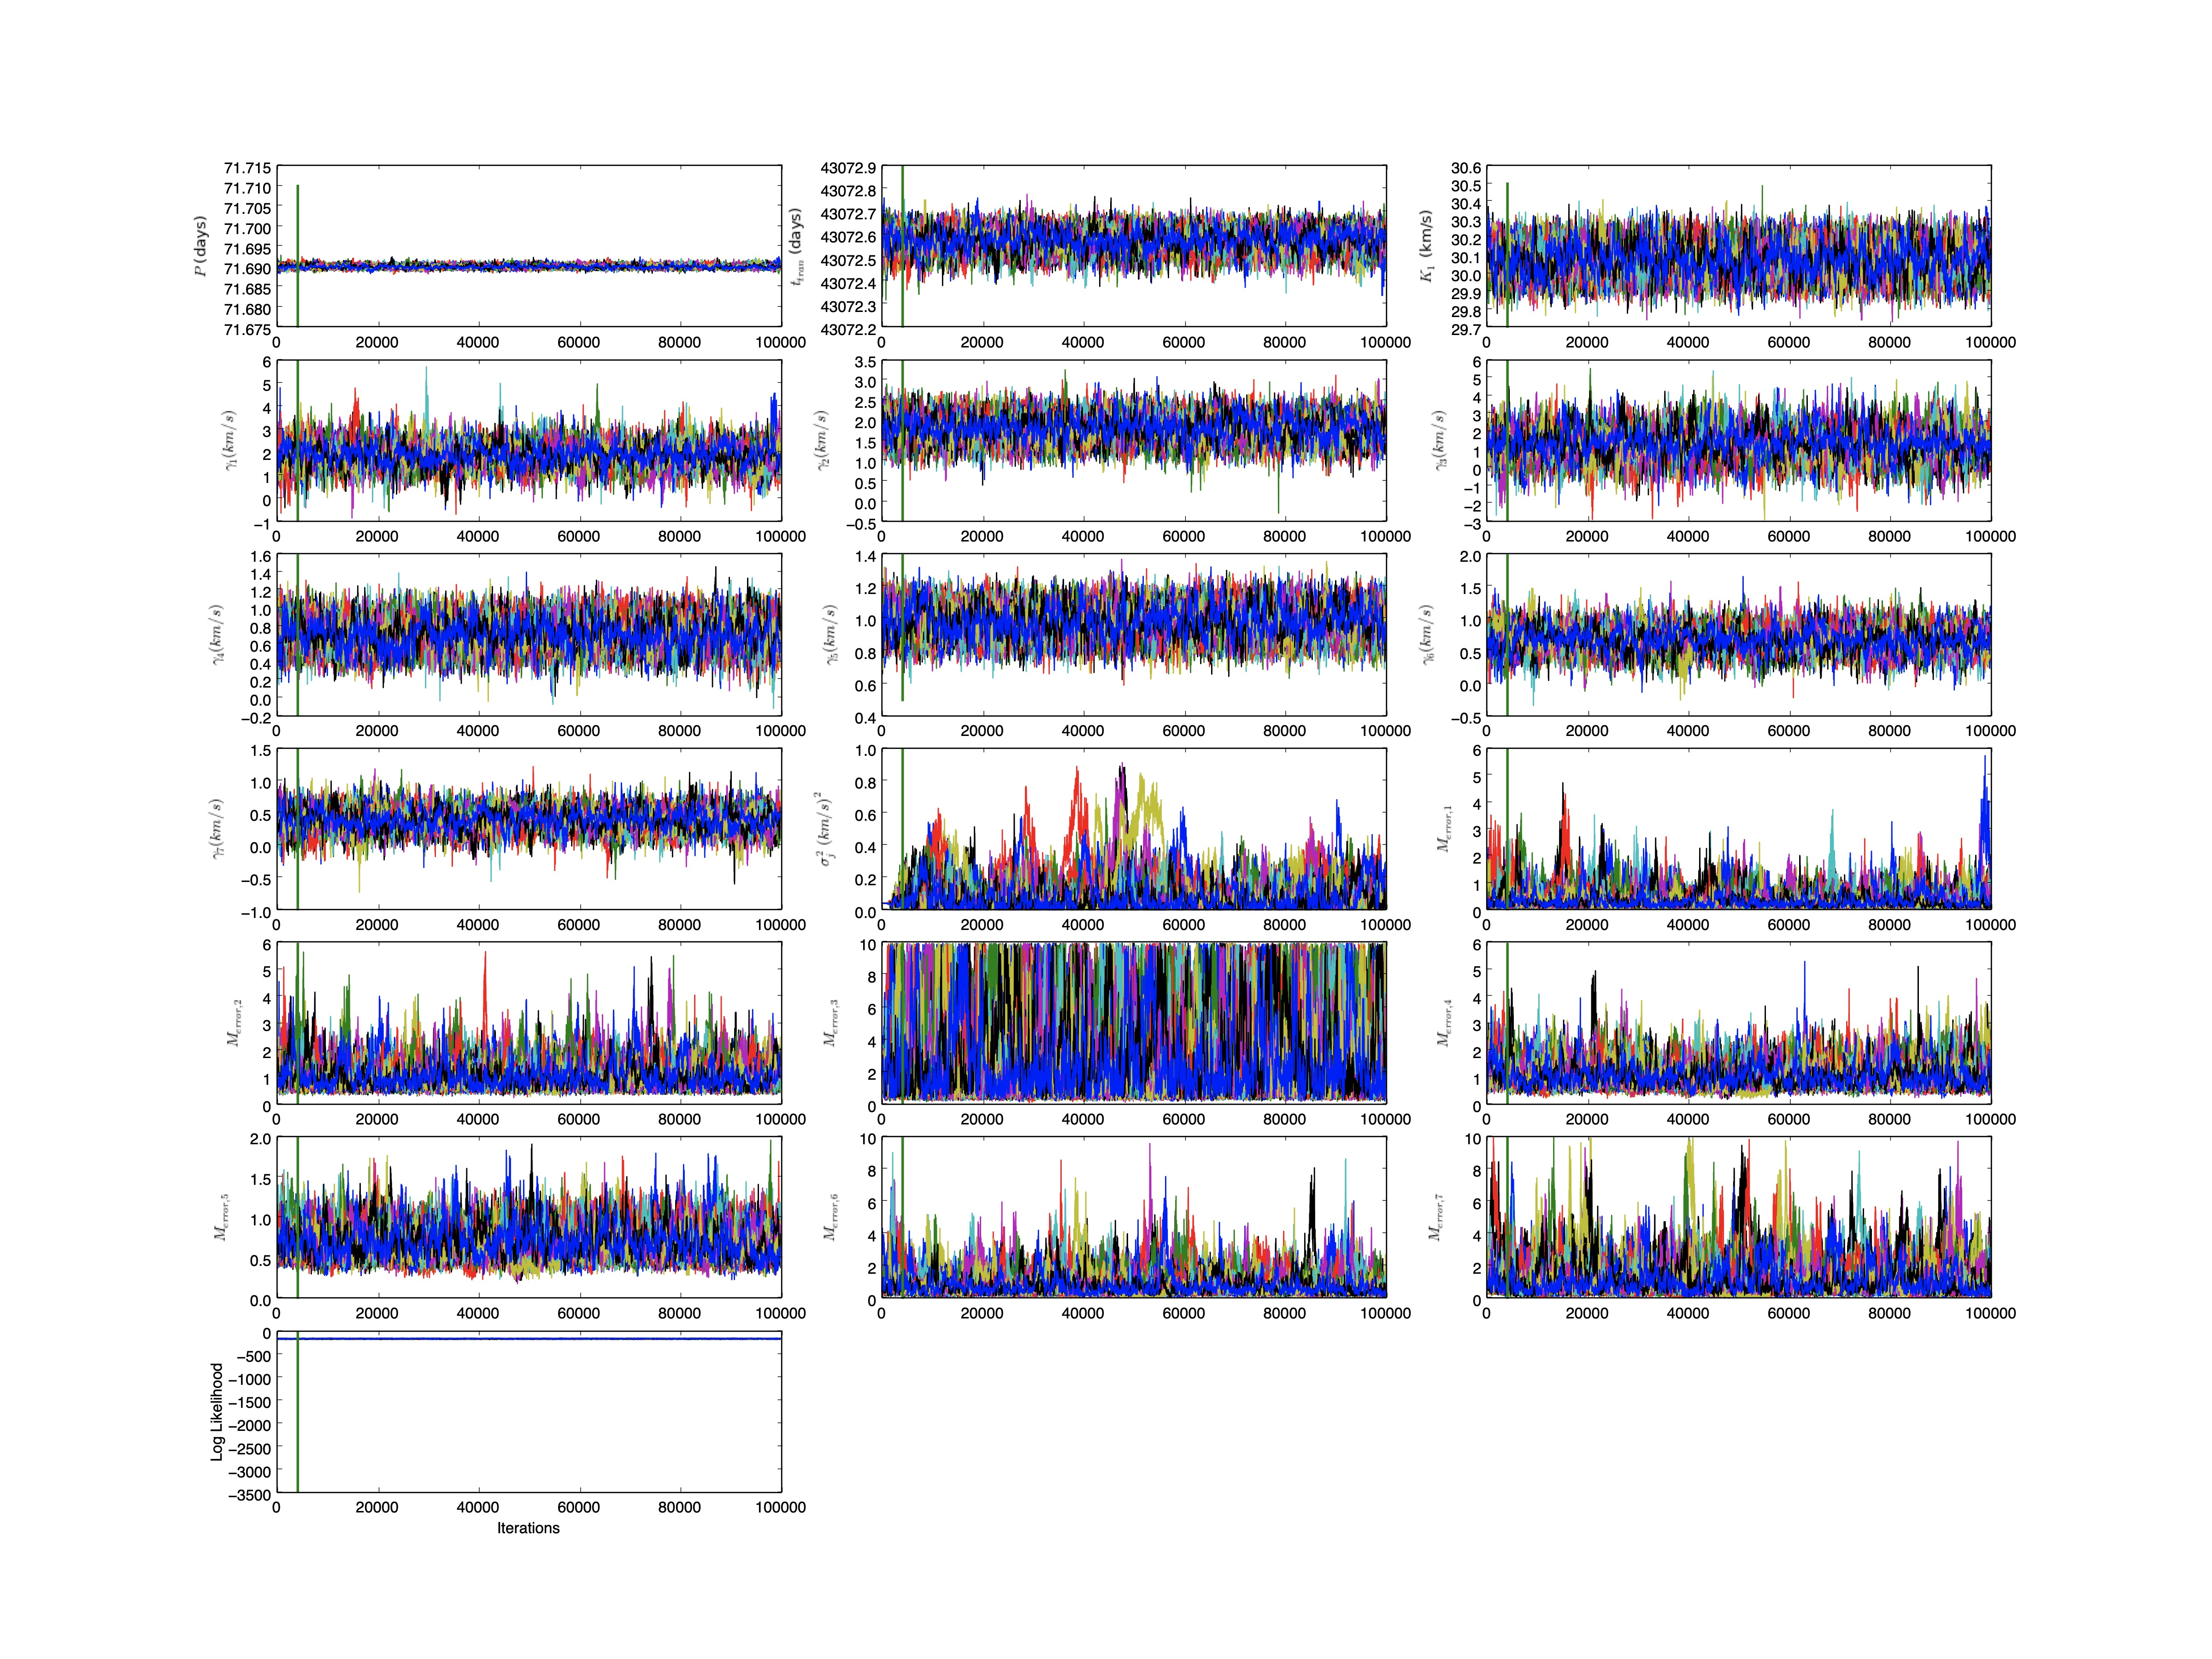
\includegraphics[width=\textwidth]{chainPlot_100000_FixedEcc.jpg}
\caption{MCMC chains for all 50 walkers. Green line is burnout: 4000 steps.}
\end{figure}

\end{document}